\documentclass[12pt]{article}
\usepackage{geometry}
\geometry{margin=1in}
\usepackage{graphicx}
\usepackage{listings}
\usepackage{color}
\usepackage{caption}
\usepackage{hyperref}
\usepackage{enumitem}
\usepackage{titlesec}

\definecolor{codegray}{gray}{0.95}
\lstset{
    backgroundcolor=\color{codegray},
    basicstyle=\ttfamily\footnotesize,
    breaklines=true,
    frame=single,
    showstringspaces=false,
    tabsize=4
}

\title{\textbf{Normalized Database Design for a Media Streaming Platform}}
\author{Student Name: Mahla Entezari \\
Course: Databases - Fall 2024 \\
Instructor: Dr. Mehrdad Ahmadzadeh Raji}
\date{\today}

\begin{document}

\maketitle

\section*{1. Project Overview}
This project involves the design, normalization, and implementation of a relational database system for a media streaming service. The goal is to create a robust and efficient schema using the Entity-Relationship (ER) model, ensure normalization up to 2NF, and implement the system in PostgreSQL using SQL commands.

\section*{2. EER Diagrams}
The conceptual model was developed using Enhanced Entity-Relationship (EER) diagrams to represent entities such as Users, Media, Subscription, Ratings, and Comments, along with their relationships.

\subsection*{2.1 EER Diagram Part 1}
\begin{figure}[h!]
    \centering
    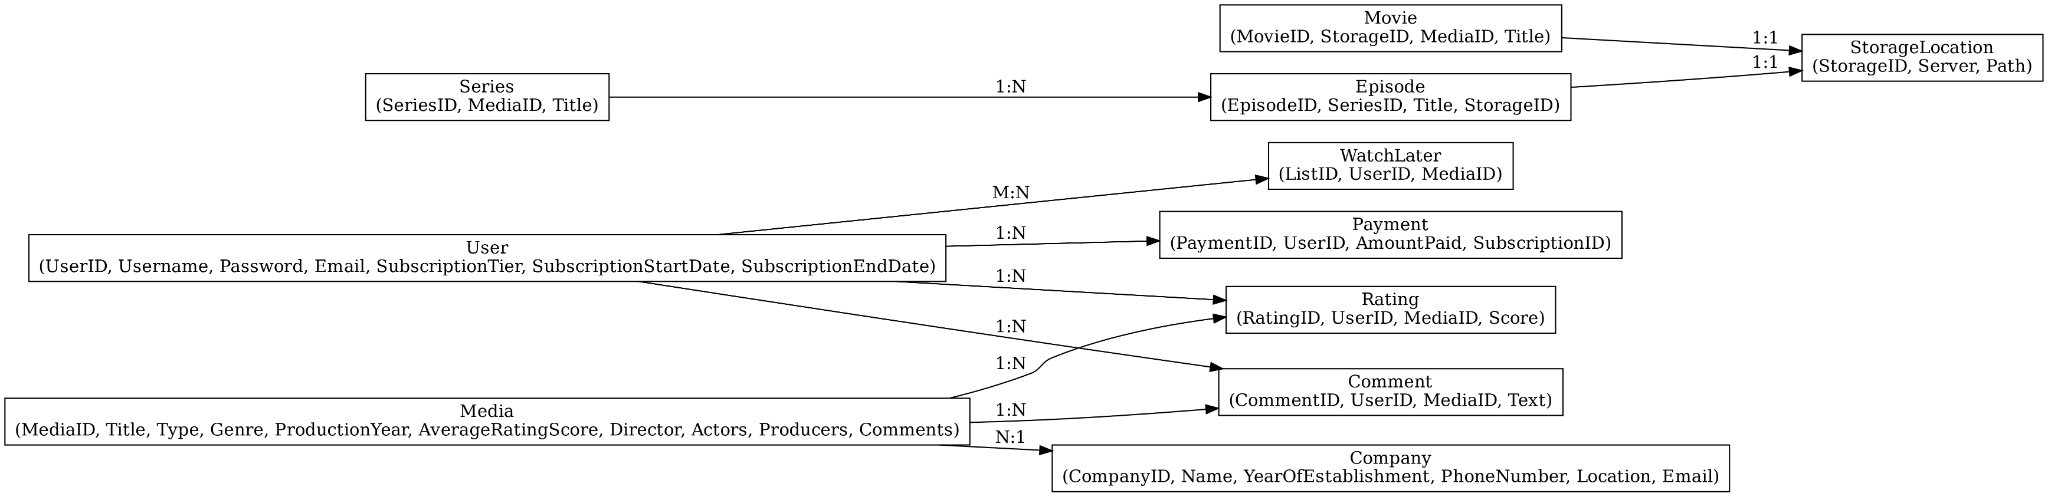
\includegraphics[width=0.85\textwidth]{eer1_converted.jpg}
    \caption{EER Diagram - User, Subscription, Media, and Comments}
\end{figure}

\subsection*{2.2 EER Diagram Part 2}
\begin{figure}[h!]
    \centering
    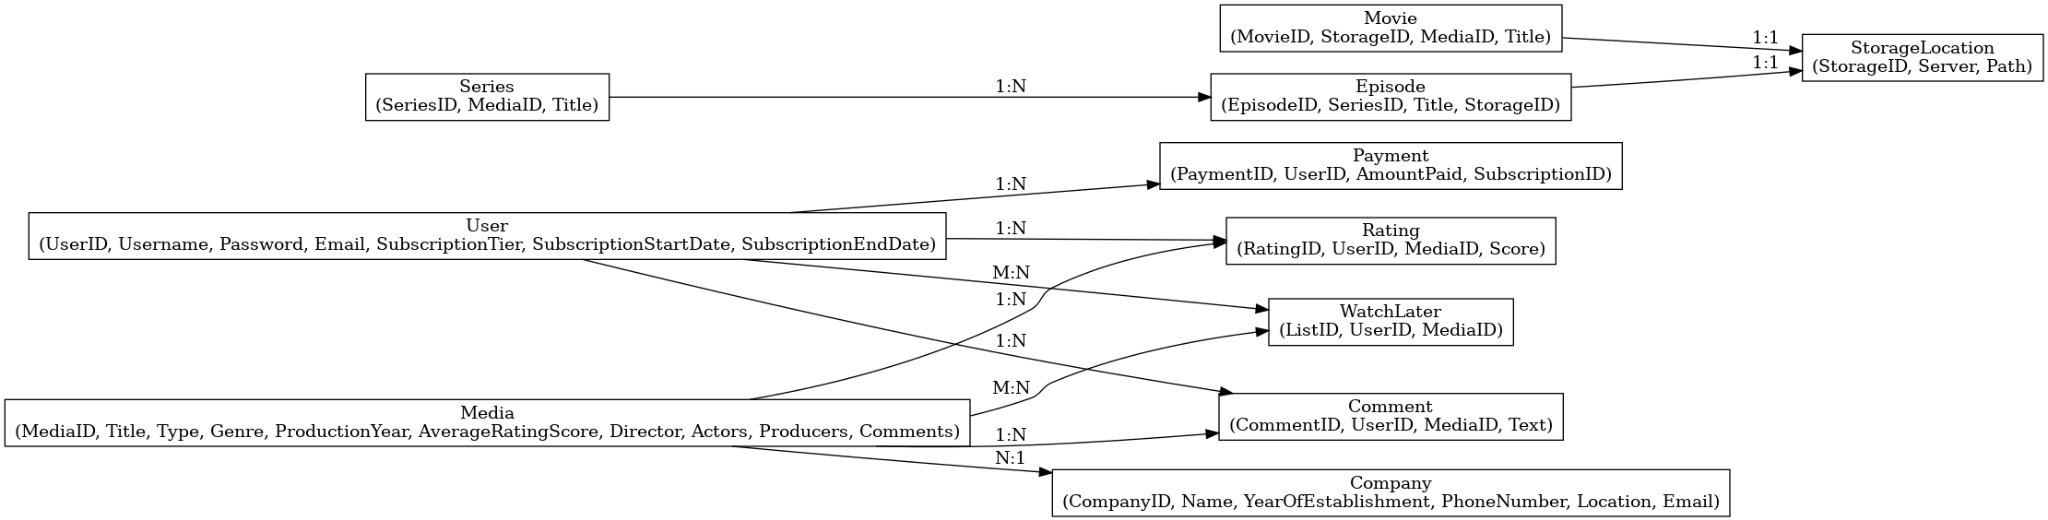
\includegraphics[width=0.85\textwidth]{eer2_converted.jpg}
    \caption{EER Diagram - Episodes, Movies, Series, and Storage}
\end{figure}

\newpage
\section*{3. First Normal Form (1NF)}
To satisfy 1NF:
\begin{itemize}
    \item All attributes must be atomic.
    \item No multivalued or composite attributes are allowed.
\end{itemize}

In our initial schema, fields like `Actors`, `Producers`, and `Comments` were stored as text arrays. To convert to 1NF:
\begin{itemize}
    \item Created separate tables: \texttt{MediaActor(MediaID, Actor)}, \texttt{MediaProducer(MediaID, Producer)}, \texttt{Comment(CommentID, UserID, MediaID, Text)}.
\end{itemize}

This ensured atomicity and removed repeating groups.

\section*{4. Second Normal Form (2NF)}
2NF requires:
\begin{itemize}
    \item Schema already in 1NF.
    \item No partial dependency of non-key attributes on part of a composite primary key.
\end{itemize}

In the 1NF schema, `SubscriptionTier`, `StartDate`, and `EndDate` depended only on `UserID` in a table where the composite key could include other fields like `PaymentID`.

To fix this:
\begin{itemize}
    \item Created a new table \texttt{Subscription(SubscriptionID, UserID, Tier, StartDate, EndDate)}.
    \item Updated related tables to remove redundant fields.
\end{itemize}

\section*{5. SQL Schema Overview}
The normalized schema is implemented in PostgreSQL using SQL. Below is a sample:

\begin{lstlisting}[language=SQL]
CREATE TABLE Users (
    UserID SERIAL PRIMARY KEY,
    Username VARCHAR(255),
    Email VARCHAR(255),
    Password VARCHAR(255)
);

CREATE TABLE Subscription (
    SubscriptionID SERIAL PRIMARY KEY,
    UserID INT REFERENCES Users(UserID),
    Tier VARCHAR(50),
    StartDate DATE,
    EndDate DATE
);

CREATE TABLE Media (
    MediaID SERIAL PRIMARY KEY,
    Title VARCHAR(255),
    Genre VARCHAR(100),
    Type VARCHAR(50),
    ProductionYear INT,
    Director VARCHAR(255)
);
\end{lstlisting}

\section*{6. Sample Advanced SQL Queries}

\subsection*{6.1 Top 5 Most Watched Media}
\begin{lstlisting}[language=SQL]
SELECT m.Title, COUNT(*) AS Views
FROM WatchHistory w
JOIN Media m ON w.MediaID = m.MediaID
GROUP BY m.Title
ORDER BY Views DESC
LIMIT 5;
\end{lstlisting}

\subsection*{6.2 User Activity in Last 30 Days}
\begin{lstlisting}[language=SQL]
SELECT u.Username, m.Title, w.Timestamp
FROM WatchHistory w
JOIN Users u ON w.UserID = u.UserID
JOIN Media m ON w.MediaID = m.MediaID
WHERE w.Timestamp >= NOW() - INTERVAL '30 days';
\end{lstlisting}

\subsection*{6.3 Average Rating per Genre}
\begin{lstlisting}[language=SQL]
SELECT Genre, AVG(Score) AS AvgRating
FROM Media m
JOIN Rating r ON m.MediaID = r.MediaID
GROUP BY Genre;
\end{lstlisting}

\section*{7. Conclusion}
This project demonstrates the transformation of a conceptual EER model into a relational schema, normalized to 2NF, and implemented in PostgreSQL. The structured design ensures data consistency, removes redundancy, and supports powerful SQL queries for media streaming insights.

\end{document}
